
%(BEGIN_QUESTION)
% Copyright 2010, Tony R. Kuphaldt, released under the Creative Commons Attribution License (v 1.0)
% This means you may do almost anything with this work of mine, so long as you give me proper credit

Large shut-off valves used on oil and gas pipelines are often opened and closed by electric valve actuators.  Such valve actuators are often used in remote locations where other sources of power such as compressed air are not available.  Electric valve actuators are also frequently used in water treatment facilities, both for actuating valves and also large gates, weirs, and other water-directing machinery.

Examine the schematic diagram on page 21 of the Limitorque L120 series actuator (L120-10 through L120-40) manual published by FlowServe (document FCD LMENIM1201-01, 07/06), and answer the following questions:

\vskip 10pt

Identify how the direction of the motor's rotation is controlled.  Specifically, explain what must happen to make the motor spin in the ``open'' direction versus the ``closed'' direction.

\vskip 10pt

Explain what the lettered ``taps'' on the control power transformer (CPT) are used for.  Under what circumstances do you think a technician would need to change the tap connections here, if ever?

\vskip 10pt

Just to the left of each motor contactor coil is a normally-closed contact linked to the {\it other} contactor.  Explain the purpose of these contacts.

\vskip 10pt

How does each contactor latch itself in and keep running after its respective ``start'' pushbutton switch has been released?

\vskip 10pt

Identify how to wire ``remote'' Stop, Open, and Close pushbutton switches to this actuator, so that it may be operated from a remote location instead of directly at the actuator.

\vskip 20pt \vbox{\hrule \hbox{\strut \vrule{} {\bf Suggestions for Socratic discussion} \vrule} \hrule}

\begin{itemize}
\item{} What advantages do electrically-actuated valves enjoy over pneumatically-actuated valves, besides not needing a compressed air supply?
\item{} What advantages do pneumatically-actuated valves enjoy over electrically-actuated valves?
\item{} Suppose a model L120 actuator were shipped to you from the factory configured for 380 volt operation.  What would you have to change in order to adapt it to work on 480 volts?
\end{itemize}

\underbar{file i02339}
%(END_QUESTION)





%(BEGIN_ANSWER)

There are two viable ways to connect the ``remote'' pushbutton switches to this electric actuator.

$$\includegraphics[width=15.5cm]{i02339x01.eps}$$

A good exercise in circuit analysis is to determine how the operation of these two connection schemes will differ.

%(END_ANSWER)





%(BEGIN_NOTES)

``Open'' contactor connects L1-T1, L2-T2, L3-T3.  ``Close'' contactor connects L1-T3, L2-T2, L3-T1 (swapping phases 1 and 3 to reverse phase rotation).

\vskip 10pt

The lettered taps on the transformer's primary winding exist to provide a means to adapt to different 3-phase power supply voltages, from 380 VAC to 500 VAC (transformer type 1).

\vskip 10pt

The NC ``O'' and ``C'' contacts are {\it interlocking} contacts, designed to prevent the two directional contactors from simultaneously energizing.

\vskip 10pt

Seal-in is accomplished by means of the NO contacts fed by the purple wire, connected respectively in parallel with pushbuttons PB1 and PB3.

\vskip 10pt

For remote operation, connect NC ``Stop'' switch between terminals 3 and 4; connect NO ``Open'' switch between terminals 1 and 3; connect NO ``Close'' switch between terminals 2 and 3: 

$$\includegraphics[width=15.5cm]{i02339x01.eps}$$

The difference between the two connection schemes shown in the answer is that ``A'' will allow an operator to jog the MOV by holding the Stop button while momentarily pressing either the Open or Close button.  Connection ``B'' does not allow for this, since holding the Stop button prevents all motion.


\vskip 20pt \vbox{\hrule \hbox{\strut \vrule{} {\bf Virtual Troubleshooting} \vrule} \hrule}

This question is a good candidate for a ``Virtual Troubleshooting'' exercise.  Presenting the diagram to students, you first imagine in your own mind a particular fault in the system.  Then, you present one or more symptoms of that fault (something noticeable by an operator or other user of the system).  Students then propose various diagnostic tests to perform on this system to identify the nature and location of the fault, as though they were technicians trying to troubleshoot the problem.  Your job is to tell them what the result(s) would be for each of the proposed diagnostic tests, documenting those results where all the students can see.

During and after the exercise, it is good to ask students follow-up questions such as:

\begin{itemize}
\item{} What does the result of the last diagnostic test tell you about the fault?
\item{} Suppose the results of the last diagnostic test were different.  What then would that result tell you about the fault?
\item{} Is the last diagnostic test the best one we could do?
\item{} What would be the ideal order of tests, to diagnose the problem in as few steps as possible?
\end{itemize}


%INDEX% Reading assignment: Limitorque L120 electric valve actuator manual

%(END_NOTES)


